% Setup - do not change
\documentclass[11pt]{article}
\usepackage[top=0.9in, left=0.9in, bottom=0.9in, right=0.9in]{geometry} 
\usepackage{parskip}

\usepackage[english]{babel}
\usepackage[utf8]{inputenc}
\usepackage{amsmath,amsthm,amssymb,graphicx,pdfpages,lipsum,hyperref}
\usepackage[none]{hyphenat}
\usepackage{csquotes}

\setlength\parindent{0pt}
%%%%%%%%%%%%%%%%%%%%%%%%%%%%%%%%%%%%%%%%%%%%%%%%%%%%%%%%%%%%%%%%%%%
% Add other packages here if required
\usepackage{multicol}
\usepackage{booktabs}
\usepackage{tabularx}

%% Bibliography is specified in this file. You can also choose an inline bib style if you want to. But make sure your citation style is consistent (and proper)
% For more details on citation: https://library.unimelb.edu.au/recite
\usepackage[sorting = none]{biblatex}
\addbibresource{references.bib}

%%%%%%%%%%%%%%%%%%%%%%%%%%%%%%%%%%%%%%%%%%%%%%%%%%%%%%%%%%%%%%%%%%% 

\title{\textbf{Maximizing Profit of NYC Yellow Taxi Driver at JFK}}
\author{
Anh Phi Vu \\
Student ID: 1266276 \\
\href{https://github.com/MAST30034-Applied-Data-Science/mast30034-project-1-anhphivu}{Github repository with commit}
}

\begin{document}
\maketitle

\section{Introduction}
In the bustling streets of New York City, the iconic yellow taxis are not only a symbol of urban movement but also a testament to the hard work of numerous drivers. For these drivers, every dollar counts, and the tips they receive significantly impact their overall earnings. Particularly at major transit hubs like the JFK International Airport, tips can make up a substantial portion of a driver's income. Recognizing this, our report aims to recommend strategies and practices that NYC yellow taxi drivers can employ to maximize tip amounts when serving passengers from JFK, leading to increased profits.

\subsection{Timeline}
The data under analysis is from a three-month period, from January 2020 to March 2020. This short yet intense window captures the heart of winter and early spring in NYC, periods known for their unique travel and tipping patterns.

\subsection{Type of Licensed Taxi}
Our lens focused on the iconic yellow taxis of NYC. Owing to their iconic status, these taxis often become the preferred choice for a wide variety of passengers, influencing tipping behaviours.

\subsection{The Data}
The data is obtained from Taxi and Limousine Commission (TLC) website \cite{taxidata} which provides a taxi trip record with attributes capturing relevant information about a taxi trip. In our research on identifying key factors affecting the tip amount, the analysis will encompass trip distance, fare amount, surcharge and indicator variables on hour time bins.

In addition, flight data within the US are used to support the analysis on maximizing tip amount for the driver. The data is obtained from the US Department of Transportation \cite{flightdata}.

\subsection{Target Audience}
While NYC yellow taxi drivers remain the primary audiences of this analysis, fleet managers, taxi associations, and platform developers might also gain valuable insights to amplify their strategies in tip maximization.

\subsection{Methodology Overview}
The analysis hinges on two robust regression techniques: Linear Regression and Random Forest Regression. Initially, the Linear Regression model will be deployed to identify and quantify relationships between independent variables and tip amounts. In parallel, the Random Forest Regression, with its ensemble of decision trees, will be employed to capture intricate, non-linear patterns that might escape the linear model. This approach ensures comprehensive coverage, offering drivers actionable insights and strategies to boost tip amounts during their JFK pickups.

\section{Data Preprocessing}
\subsection{Taxi Data}
The data set comprises an extensive collection of taxi ride records over 3 months, with 15,712,062 rows and 19 columns. Given its substantial size and complexity, preprocessing is an imperative step. Proper preprocessing ensures cleaner data, enabling more accurate analysis and modelling. 
\begin{itemize}
    \item To prevent potential discrepancies during data analysis and ensure uniformity, columns' names were standardized by changing them to lowercase. 
    \item To prevent the significant impact of missing values on the overall analysis, columns with missing values are dropped. After this, the data set size reduce to 14 columns.
    \item In preventing type-related errors during analysis and modelling, the consistent data types for each column were cast. 
    \item Trips with \texttt{vendor\_id} beside 1 and 2 were removed as specified in the data dictionary \cite{taxidatadict}. 
    \item Exclude all trips with negative \texttt{trip\_distance} as travelling distance cannot be negative.
    \item Exclude all trips with \texttt{payment\_type} other than 1 because tipping only populated for credit card payment \cite{taxidatadict}. 
    \item Exclude all trips with \texttt{fare\_amount} less than \$3, the minimum fare amount set by NYC \cite{fareamount}.
    \item Only include trips with \texttt{pulocationid} 132 indicating pick up at JFK as the analysis focused on picking up passengers from JFK. 
\end{itemize}
Moreover, outlier removal was done using the IQR method due to its robustness to extreme value and applicability to non-normal distribution data. After this, the data set reduces to 269,641 rows. 

\subsection{Flights Data}
The data set comprises flight data within the US over 3 months, with 1,838,081 rows and 72 columns. Initially, the data comes in \texttt{.asc} format, with no header. An extensive preprocessing process is needed to ensure the data is usable for analysis and modelling:
\begin{itemize}
    \item Column headers were added for ease of reference during data analysis and modelling. 
    \item Unnecessary columns and columns with a substantial amount of NaN results are dropped. After this, the data set size reduce to 8 columns
    \item Consistent data types for each column were cast for the same reason as Taxi Data. 
    \item Only include flights with \texttt{arrival\_airport} JFK since it is the main focus of the analysis. 
    \item Outlier removal was done using the IQR method and reduced the data set size to 22,039 rows.
\end{itemize}

\subsection{Feature Engineer}
Feature engineering plays a pivotal role in enhancing the potential predictive power of the models by capturing additional underlying patterns in the data.

Taxi rides and the associated tips might exhibit patterns based on the hour of the day. For instance, late-night or early-morning rides might have different tipping behaviours than mid-day rides due to factors like tiredness, urgency, or fewer available taxis. Hence, both data sets have been added hourly bins columns as an indicator variable for which hour of the day the trip started or the flight landed. 

Beyond the hourly bins, \texttt{weekend}, \texttt{weekend}, and rush hours indicators have been added to the taxi data set. These are crafted to encapsulate the weekly and daily rhythms of life in New York City, which can influence taxi usage and tipping behaviours.

\section{Exploratory Analysis}
\subsection{Pick Up Trend in NYC}
Figure 1 below shows the total amount of trips picked up in each location over the period of 3 months. A clear pattern emerges that highlights the bustling activity of Manhattan, a known epicentre for taxi pickups. Yet, right outside this urban heart, JFK Airport prominently stands out as its dark orange shades on the bottom right indicate an intense frequency of taxi pickups. This underscores JFK's pivotal role as a significant hot spot for taxi drivers aiming to maximize their profit.

\begin{figure}[h]
    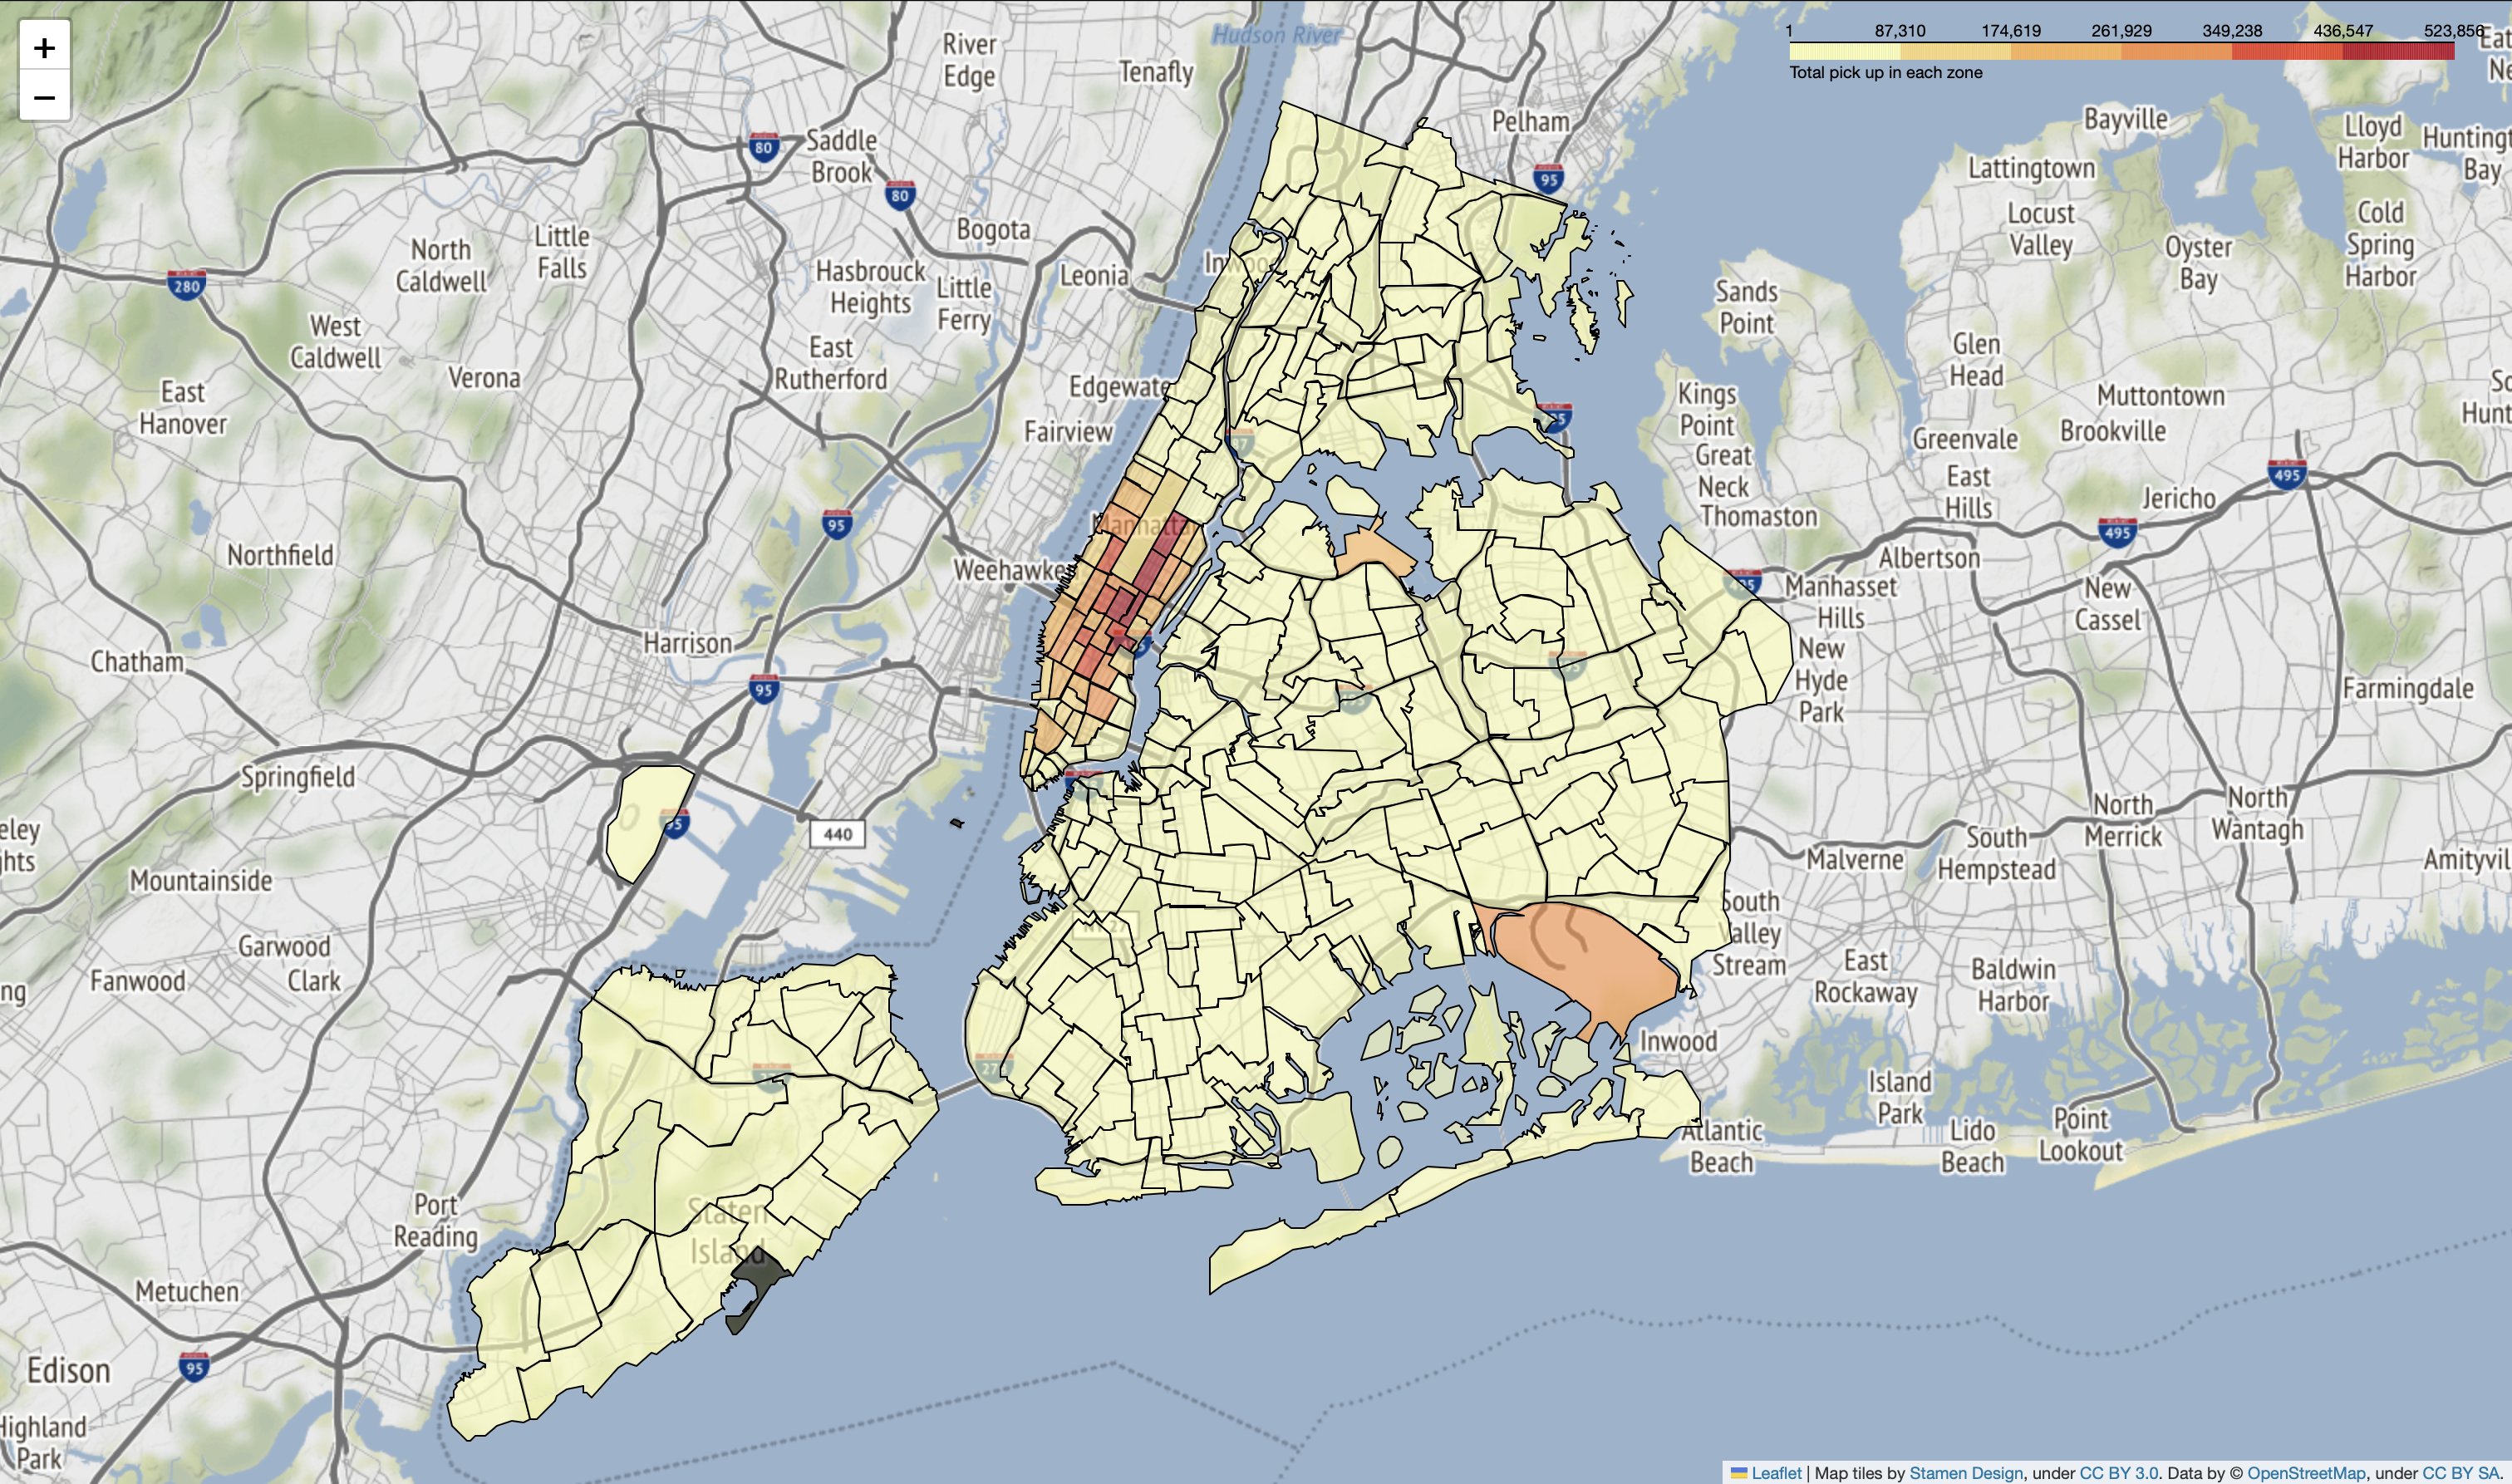
\includegraphics[width=0.8\textwidth]{plots/pickup_per_zone.png}
    \centering
    \caption{Total Pick Up per zone} 
\end{figure}

\subsection{Pick Up and Flight Arrival Trend at JFK}
Figures 2 and 3 below show the total amount of trips picked up at JFK and flights arriving at JFK over the period of 3 months in an hourly manner. From Figure 2, the golden hours for taxi drivers appear to span from the late afternoon to the early hours of the next day, between 2 pm and 1 am. This can be explained by Figure 3, the flight inflow pattern is distinctly tri-modal, with spikes observed during the early morning (6 am - 9 am), mid-afternoon (1 pm - 4 pm), and evening (6 pm - 10 pm). While first glance might suggest a misalignment between peak flight arrivals and taxi pickups, a deeper dive reveals the logic. Passengers often take a while to disembark, navigate immigration, customs, and collect baggage before they're ready for a taxi. This lag potentially explains why the surge in taxi pickups postdates the flight arrivals by a few hours. 

\begin{figure}[h]
    \centering
    \begin{minipage}{0.4\textwidth}
        \centering
        \includegraphics[width=1.0\linewidth]{plots/trips_pickup_count_JFK.png}
        \caption{Pick Up Trend at JFK}
    \end{minipage}
    \hfill
    \begin{minipage}{0.4\textwidth}
    \centering
    \includegraphics[width=1.0\linewidth]{plots/flights_arrival_count_JFK.png}
    \caption{Flights Arrival Trend at JFK}
    \end{minipage}
\end{figure}

\subsection{Distribution of Tip Amount}
One of the primary metrics directly linked to driver profitability is the tip amount. From Figure 4, the distribution of tip amount is visualized by the density plot. The majority of the tips lie in the range of \$0 to \$20 with an average of \$9.5. The density peak near the average suggests that a substantial number of passengers tend to hover around this tipping point, possibly viewing it as a 'standard' or 'acceptable' tip amount.

\begin{figure}[h]
    \includegraphics[width=0.7\textwidth]{plots/tip_amount_density_JFK.png}
    \centering
    \caption{Distribution of Tip Amount} 
\end{figure}

\section{Modelling}
Two models chosen to understand the relationship between tip amount and other variables and potentially predict the tip amount are Linear Regression (LR) and Random Forest Regression (RFR). 

\subsection{Linear Regression}
Linear Regression was chosen due to its interpretation ability and application. Using LR, we can understand how different variables linearly affect the tip amount.

Figure 5 below shows the correlation between the variables used. Indicator variables and categorical variables are not included in the heat map because the \texttt{.corr()} function in pandas will calculate the point-biserial correlation for indicator variables, which might not be as intuitive as a standard Pearson correlation. From Figure 5, the variables showcased positive correlations with each other. This indicates that as one variable increases, the other variables tend to increase as well. 

\begin{figure}[h]
    \includegraphics[width=0.5\textwidth]{plots/features_correlation_heatmap_JFK.png}
    \centering
    \caption{Features Correlation Heat Map} 
\end{figure}

However, high correlations between features might lead to multicollinearity, where variables are highly interrelated. To get a visual grasp on potential multicollinearity and underlying distributions, Figure 6 shows the pairwise plots between the features which help determine which variables to transform and avoid multicollinearity. 

\begin{figure}[h!]
    \includegraphics[width=0.5\textwidth]{plots/features_pairwise_JFK.png}
    \centering
    \caption{Pairwise Plot of Variables} 
\end{figure}

From Figure 6, there's a somewhat linear relationship between the variables, although with a lot of variance. However, \texttt{trip\_distance} seems to be right-skewed, which is a potential candidate for logarithmic transformations. \texttt{fare\_amount} share similar skewness pattern as \texttt{trip\_distance}. Taking logarithmic transformation of these two variables mitigate the effects of multicollinearity, making the model more interpretable. 

After tackling the transformation of variables, the Linear Regression model was fitted to the data. Tables 1 and 2 below show the variables with the corresponding coefficients. 

\begin{table}[h]
    \centering
    \begin{minipage}{.5\textwidth}
        \centering
        \caption{Regression Coefficients 1}
        \label{tab:coefficients1}
        \begin{tabular}{lc}
            \toprule
            Predictor & Coefficient \\
            \midrule
            const & -9.704524 \\
            log\_trip\_distance & 0.047723 \\
            log\_fare\_amount & 5.972449 \\
            weekend & -4.837108 \\
            weekday & -4.867416 \\
            morning\_rush & -0.132572 \\
            evening\_rush & 0.116423 \\
            total\_surcharge & 0.178622 \\
            {[0-1]} & 0.048335 \\
            {[1-2]} & -0.106499 \\
            {[2-3]} & -0.152673 \\
            {[3-4]} & -0.585132 \\
            {[4-5]} & -0.153019 \\
            {[5-6]} & -0.150234 \\
            {[6-7]} & -0.178816 \\
            {[7-8]} & 0.091843 \\
            \bottomrule
        \end{tabular}
    \end{minipage}%
    \begin{minipage}{.5\textwidth}
        \centering
        \caption{Regression Coefficients 2}
        \label{tab:coefficients2}
        \begin{tabular}{lc}
            \toprule
            Predictor & Coefficient \\
            \midrule
            {[8-9]} & -0.019598 \\
            {[9-10]} & -0.204817 \\
            {[10-11]} & 0.011106 \\
            {[11-12]} & 0.139551 \\
            {[12-13]} & 0.081518 \\
            {[13-14]} & 0.054960 \\
            {[14-15]} & 0.219424 \\
            {[15-16]} & 0.244560 \\
            {[16-17]} & 0.286773 \\
            {[17-18]} & 0.087184 \\
            {[18-19]} & 0.053356 \\
            {[19-20]} & -0.024117 \\
            {[20-21]} & 0.248826 \\
            {[21-22]} & 0.099863 \\
            {[22-23]} & 0.151308 \\
            \bottomrule
        \end{tabular}
    \end{minipage}
\end{table}

From table 1 and 2:
\begin{itemize}
    \item \texttt{weekend} and \texttt{weekday}: Surprisingly, trips taken during the weekday has higher tips than trips taken during the weekend by \$0.030. This can be caused by commuting patterns. During weekdays, there might be more people commuting to and from the airport for work-related reasons, resulting in more frequent and possibly longer trips.
    \item \texttt{morning\_rush} and \texttt{evening\_rush}: Trips taken during the evening rush hour make \$0.250 more in tips than trips taken during the morning rush hour. This can be due to the nature of travellers as morning commuters may be in a hurry and less attentive to the tipping process. In contrast, evening commuters, as they end the work day, can be more relaxed and generous in their tipping habits.
    \item \texttt{[16-17]}: This indicates that the trips started from JFK from 4 pm to 5 pm. The coefficient of 0.287, the higher of all hourly bins, means that trips taken during this hour time frame make \$0.287 more in tips compared to trips taken during other times keeping all factors constant.
\end{itemize}

The coefficients from the hourly bins suggest that the hours from 2 pm to 1 am the next day generally see a higher tip amount, indicated by positive coefficients. 

The afternoon flight peak from 1 pm to 4 pm and the evening flight peak from 6 pm to 10 pm align well with the higher tip amounts seen from 2 pm onwards. This suggests that as passengers disembark from their flights during peak times, taxi drivers at JFK know the opportunities for greater tips thus, they drive there to pick up passengers

However, the morning flight peak from 6 am - 9 am doesn't directly align with the higher tip amounts based on the coefficients provided. It might be that passengers arriving in the morning have alternative transportation options or that the taxi rides taken during these hours are shorter in distance, resulting in lower tips.

\subsection{Random Forest Regression}
Random Forest Regression was chosen because it can capture non-linearities and interactions between features as well as it relies on constructing multiple decision trees during training which can offer higher accuracy. 

We tune the parameter to optimize the performance of the model. Through grid search, the optimal parameters are:

\begin{itemize}
    \item \texttt{max\_depth = 10}: This prevents the model from being overly complex and mitigates overfitting. 
    \item \texttt{min\_samples\_leaf = 4}: This ensures that the trees aren't growing too deep with leaves handling very few samples, preventing overfitting. 
    \item \texttt{min\_samples\_split = 10}: This controls the growth of the trees and ensures that each internal node splits into child nodes only if it has at least 10 samples.
\end{itemize}

\section{Discussion and Evaluation}
To comprehensively evaluate the performance of our two models, LR and RFR, we use \( R^2 \), MAE (Mean Absolute Error), MSE (Mean Squared Error) and RMSE (Root Mean Squared Error). Each of these metrics provides unique insights into the model's strengths and areas of improvement.

\begin{table}[h]
    \centering
    \caption{Model Evaluation Metrics}
    \label{tab:metrics}
    \begin{tabular}{lcccc}
        \toprule
        Model & \( R^2 \) & MAE & MSE & RMSE \\
        \midrule
        Linear Regression & 0.248 & 2.591 & 14.549 & 3.814 \\
        Random Forest Regression & 0.283 & 2.540 & 13.465 & 3.670 \\
        \bottomrule
    \end{tabular}
\end{table}

From Table 3, the RFR model higher \( R^2 \) indicates that it explains the change in tip amount using the features in the model better than the LR model. The MAE of both models suggests that, on average, predictions by the two models (LR and RFR) are off by about 2.591 and 2.540 units from the actual values respectively. The MSE and RMSE value of both models indicates that both models' prediction on average, deviate from the actual value by fairly similar number. 

While both models are fairly close in terms of performance, the Random Forest Regression model exhibits slightly better accuracy across all metrics. The \( R^2 \) of below 0.3 for both models suggests that there may be other important variables or interactions not captured by the models. However, from the actual vs. predicted value plots for the RFR model in Figure 7 below, the models' predictions are fairly accurate for low tip amounts as the majority of data points cluster around the average. 

\begin{figure}[h]
    \includegraphics[width=0.65\textwidth]{plots/predicted_vs_actual_RFR.png}
    \centering
    \caption{Actual vs. Predicted Values} 
\end{figure}

\section{Recommendations}
After thorough analysis and exploration of the NYC Yellow Taxi data, specific patterns and trends emerge that can guide taxi drivers in making informed decisions to optimize their earnings. 

Taxi drivers looking to maximize their profit should prioritize their presence at JFK during the mid-afternoon and evening rush. Given the flight arrival pattern, it's evident that these are peak times when passengers would require taxi services the most. By ensuring availability during these peak inflow times, taxi drivers can increase their chances of securing a good tip.

While JFK remains a priority, taxi drivers should also consider catering to the weekday evening rush outside the airport. This could involve transporting working professionals or city visitors during their evening outings. The data suggests that such trips not only have a higher frequency but also yield better tips, making them a profitable option for drivers.

\section{Conclusion}
In conclusion, the study of maximizing profits for NYC Yellow Taxi drivers operating around JFK embarked on a comprehensive analysis of taxi trip data, spanning from January to March 2020. By delving deep into the data, we reveal vital patterns surrounding pick-up hotspots, trip timings, and tip amounts. Through the modelling approaches, namely Linear Regression and Random Forest Regression, we gained an understanding of the factors most affecting profitability. These findings not only offer a clear picture of the taxi landscape around JFK but also serve as a road map for drivers aiming to increase their earnings via tip. In an evolving urban transport landscape, such data-driven insights become indispensable tools for taxi drivers, ensuring that they remain competitive and continue to serve the city's residents and visitors effectively. 

\clearpage
\printbibliography
\end{document}